\chapter{Grundlagen}
\label{sec:Grundlagen}
Leistungselektronik befasst sich mit der Umwandlung und Steuerung elektrischer Energie, um sie effizient in verschiedenen Formen für elektronische Geräte und Systeme nutzbar zu machen. Insbesondere die Entscheidung zwischen Wechsel- und Gleichstrom in den Übertragungs- und Verteilungsnetzen bleibt eine Debatte. Mit der Weiterentwicklung der Halbleitertechnik zeigt sich, dass die Gleichstromtechnik auch bei langen Übertragungsstrecken Vorteile gegenüber der verbreiteten Wechselstromtechnik hat. Um die Anforderungen und Zusammenhänge verstehen zu können, werden Details zur Elektrolyse, zu Stromrichtern und Komponenten sowie zur verwendeten Simulationsumgebung vorgestellt.
\section{Wasserstoff-Elektrolyse}
\label{sec:Elektrolyse}
Das Prinzip der \gls{AEL} ist, im Gegensatz zur neueren \gls{PEM} Elektrolyse, bereits seit langem bekannt und optimiert. Die \gls{AEL} benötigt in der Regel eine wässrige Kalilauge und kann durch Reihenschaltung der Zellen Wasserstoff und Sauerstoff unter erhöhtem Druck von z.~B. 30 bar bereitstellen. Die Entwicklung und insbesondere die Steigerung der Stromdichte und des Wirkungsgrades haben in den letzten Jahren keine großen Veränderungen gebracht. Der Spannungswirkungsgrad liegt zwischen 62 und 82 Prozent \cite{NOWH2}. Der Spannungswirkungsgrad bei der Elektrolyse von Wasserstoff bezieht sich auf das Verhältnis zwischen der tatsächlich benötigten elektrischen Spannung und der theoretisch erforderlichen Spannung, um Wasser in Wasserstoff und Sauerstoff zu spalten. Dieser kann im Verhältnis zur Stromdichte aufgetragen werden und bietet damit eine Übersicht über die Effizienz und Stromdichte, siehe Abbildung \ref{fig:ely-efficiency}. Die Stromdichte ist eine Vergleichsgröße für die benötigte Elektrodenfläche, den Platzbedarf und die benötigten Materialmengen.\\
Die \gls{PEM}-Elektrolyse bietet Vorteile durch erhöhte Stromdichte, bei größeren Anlagen spart dies unter anderem Platz, außerdem ist zu erwarten, dass Druckelektrolyse bis 100 bar möglich wird. Dies erhöht den Gesamtwirkungsgrad, da die Elektrolyseure den hohen Druck für die Lagerung oder den Transport generieren und somit Kompressoren eingespart werden können. Optimierungsbedarf besteht jedoch noch bei der Lebensdauer der Membranen und den benötigten Edelmetallen \cite{NOWH2}. \\
Die \gls{HTEL} nutzt die Vorteile höherer Temperaturen von oft über 500 °C, die thermodynamische Vorteile für den elektrischen Wirkungsgrad bringen, jedoch hohe Anforderungen an die verwendeten Materialien stellen. Sie wird auch als Hochtemperatur-Wasserstoff-Festoxid-Elektrolysezelle (SOEC) bezeichnet. Der Name "Festoxid" bezieht sich auf die Art der Elektrolyten in der Zelle. In SOECs werden feste keramische Materialien als Elektrolyten verwendet, typischerweise aus Zirkonoxid (ZrO2) oder Yttrium-stabilisiertem Zirkonoxid (YSZ). Die Technologie der Festoxidelektrolyse befindet sich noch im Stadium der Grundlagenforschung im Labor. Da fast alle Festoxidzellen reversible Eigenschaften besitzen, ist das Interesse an ihnen besonders groß, da dies eine direkte Rückverstromung des Wasserstoffs ermöglicht. Allerdings sind auch hier noch Materialoptimierungen und Verbesserungen der Langzeiteigenschaften notwendig.\\
\begin{figure}
	\centering
	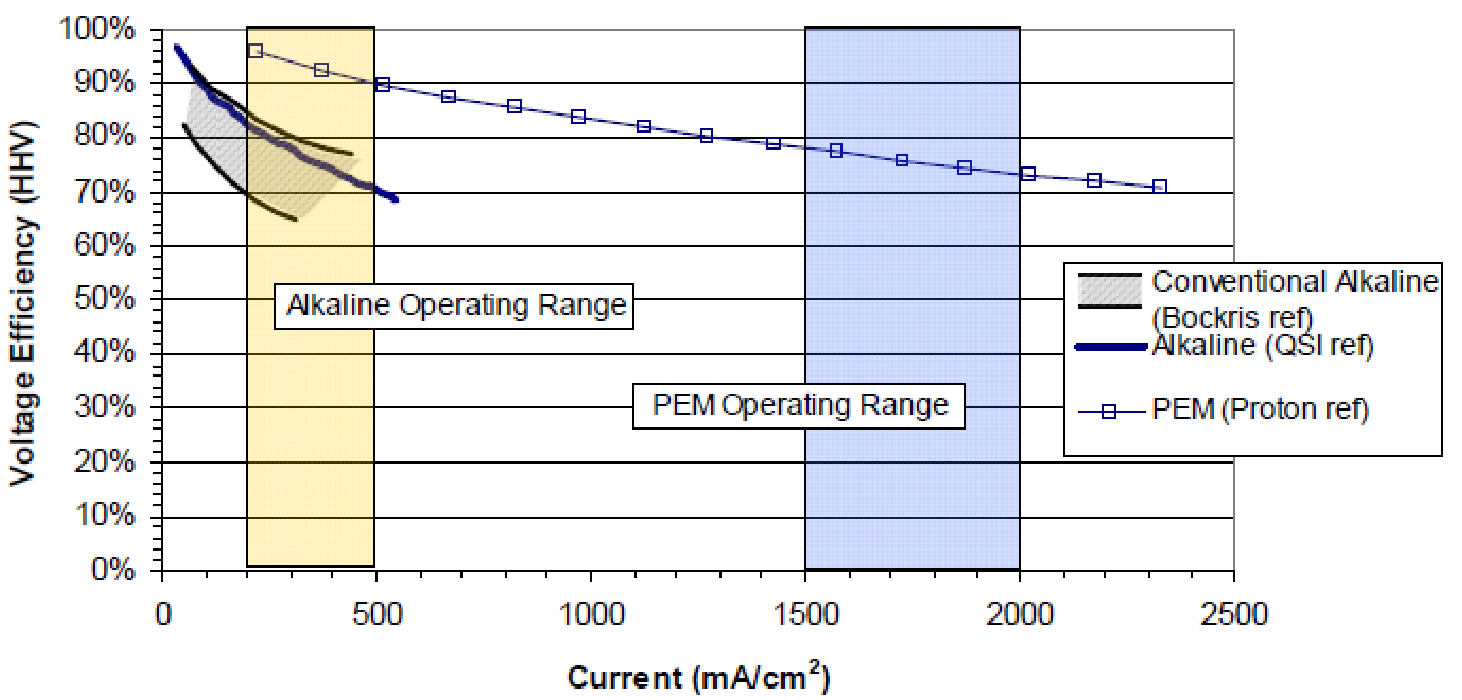
\includegraphics[width=0.9\linewidth]{content/Grafiken/Ely-Efficiency}
	\caption{Elektrolyseur Spannungseffizienz \cite{NOWH2}}
	\label{fig:ely-efficiency}
\end{figure}
\section{Stromrichter}
\label{sec:Stromrichter}
Allgemein kann jede Schaltung zur Strom- und Spannungsversorgung als Stromrichter bezeichnet werden, wobei zwischen AC- und DC-Varianten unterschieden wird. Weiterhin kann bei Netzanwendungen zwischen geregelt, netzgeführt und ungesteuert unterschieden werden, sowie die Implementierung einer \gls{PFC} betrachtet werden \cite{Schroder.2018}.  
		\subsection{Gleichrichter}
		\label{sec:Rec}
		Ein Gleichrichter wird genutzt, um aus einer Wechselspannung eine Gleichspannung zu erzeugen. Die einfachste Form ist der Diodengleichrichter. Dieser kann für einphasige Wechselspannung durch eine einzelne Diode realisiert werden. Allerdings würde so nur die halbe Periode des Sinus am Ausgang zur Verfügung stehen, da die Diode nur während der positiven Halbwelle leitet. Dies kann durch die Ergänzung eines Brückengleichrichters mit vier Dioden für einphasige Anwendungen und sechs Dioden für dreiphasige Anwendungen erreicht werden. Der Dreiphasige Diodengleichrichter findet sich in Abbildung \ref{fig:B6DiodRect}.\\
		\begin{figure}
			\centering
			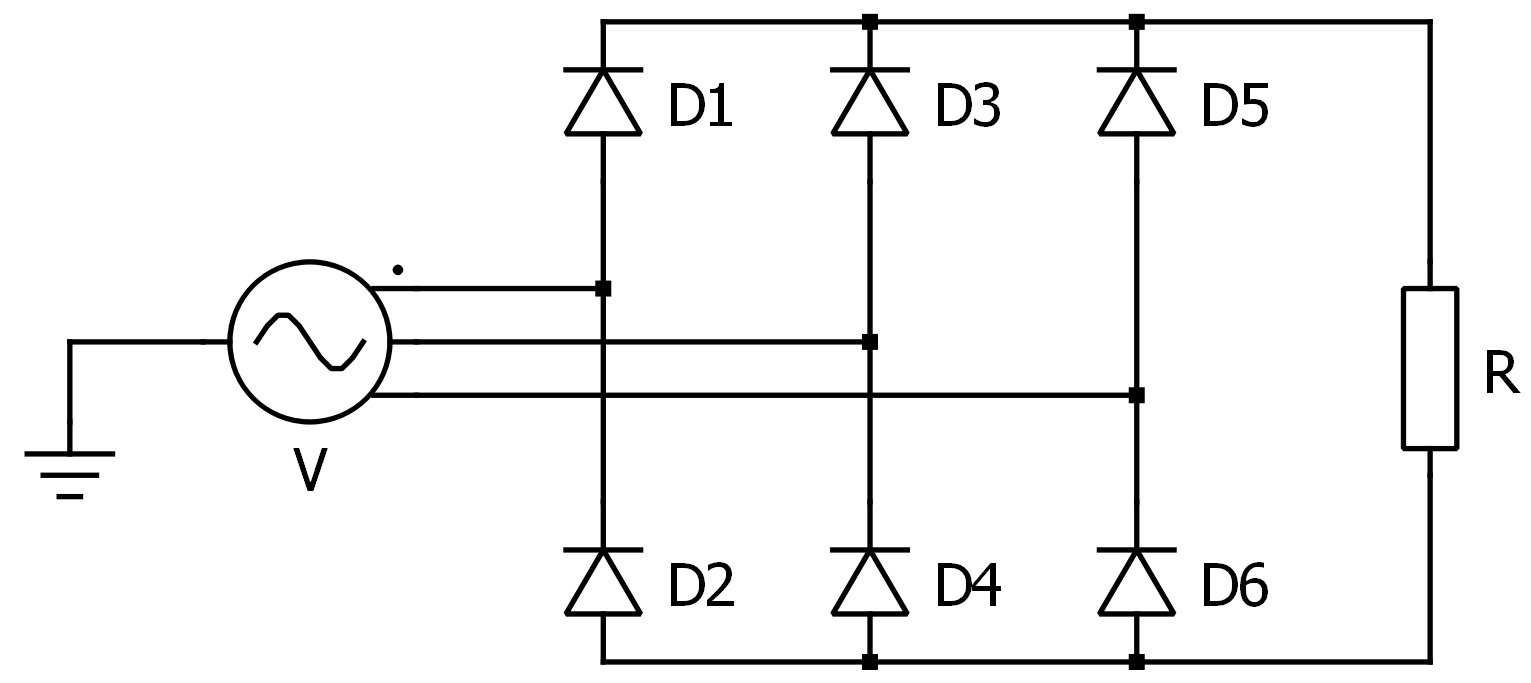
\includegraphics[width=0.8\linewidth]{content/Grafiken/Plecs_Diodengleichrichter}
			\caption{Diodengleichrichter für Dreiphasige Anwendungen}
			\label{fig:B6DiodRect}
		\end{figure}
		Der Diodengleichrichter ist jedoch nur bedingt für einen gewünschten Stromverlauf geeignet. In Abbildung \ref{fig:B6DiodRectI} ist der Netzspannungs und Stromverlauf des Diodengleichrichter dargestellt. Der Stromverlauf zeigt starke Sprünge und der gewünschte sinusförmige Verlauf ist nur schwer erkennbar, dies kann durch Ergänzung von Kondensatoren und Spulen zur Filterung teilweise korrigiert werden. Außerdem ist es mit dieser Schaltung nicht möglich, die Ausgangsspannung oder den Strom zu variieren.\\
		\begin{figure}
			\centering
			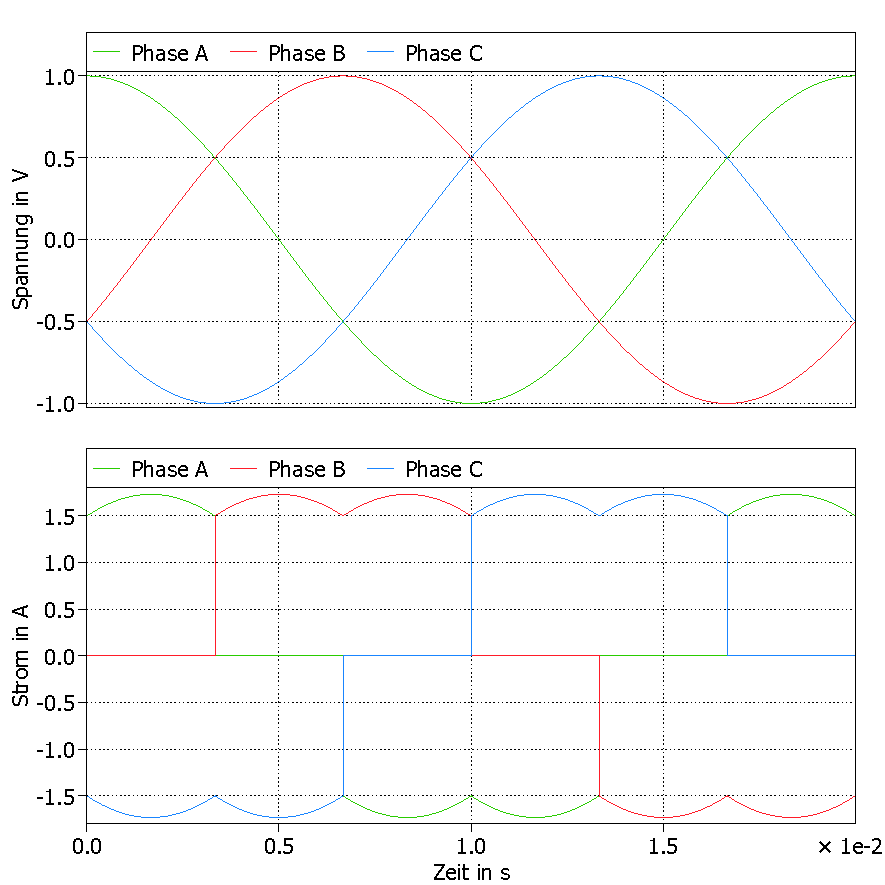
\includegraphics[width=0.65\linewidth]{content/Grafiken/B6-Diodengleichrichter-Eingangsverlauf}
			\caption{Strom und Spannungsverlauf des Dreiphasigen Diodengleichrichters }
			\label{fig:B6DiodRectI}
		\end{figure}
		Dioden- sowie Thyristorgleichrichter lassen sich in großen Leistungsklassen zentral aufbauen, bieten jedoch oft nicht die nötige Flexibilität. Für Elektrolyseanlagen mit mehreren Megawatt Leistung und gewünschter Netzdienlichkeit ist eine Parallelisierung der Leistungshalbleiter notwendig, da bei Spannungen bis 1000 V die Ströme für einzelne Halbleiter zu hoch sind. Beispielsweise Infineon bietet derzeit in der 2000 Volt \gls{SiC}-\gls{MOSFET} Reihe Module mit einem Nennstrom bis 400 Ampere an. Dies reicht bei einer Ausgangsleistung von einem Megawatt und einer Ausgangsspannung von 1 kV nicht aus, um die benötigten 1 kA zu erreichen. \\
		Mit thyristorbasierten Schaltungen können große Leistungen effizient umgesetzt werden, allerdings führen sie zu deutlichen Verzerrungen im Stromverlauf und zu einem schlechteren Leistungsfaktor. Sie erfordern daher passive oder aktive Filter, die die Systemkosten erhöhen \cite{HydrogenElectronicTopologies}. Die Parallelisierung durch Interleaving und Phasenverschiebung bietet deutliche Vorteile durch geringere Verzerrung und damit weniger Filteraufwand. \\
		Als Alternative werden \gls{AFE} Gleichrichter eingesetzt, die wesentlich geringere Verzerrungen und Freiheit bei der Regelung des Eingangsstroms bieten. Filter fallen deutlich kleiner aus und auf Blindleistungskompensation kann in diesem Fall verzichtet werden \cite{HydrogenElectronicTopologies}.
		\subsection{DC-DC Wandler} \label{sec:Buck}
		Der Hochsetzsteller und der Tiefsetzsteller sind grundlegende Topologien, die im Wesentlichen aus zwei Halbleitern und einer Induktivität bestehen. In Abb. \ref{fig:buck} ist die Schaltung eines Tiefsetzstellers dargestellt. Über die \gls{D} des Schalters kann die \gls{Ua} eingestellt werden, wobei die Parameter \gls{Ue}, Lastimpedanz sowie der Wert der Induktivität relevant sind. Die Ausgangsspannung kann für den Betrieb ohne Unterbrechung über die Beziehung $U_{out}=D\cdot U_{in} $ berechnet werden \cite{schmidtwalter}.
		\begin{figure}
			\centering
			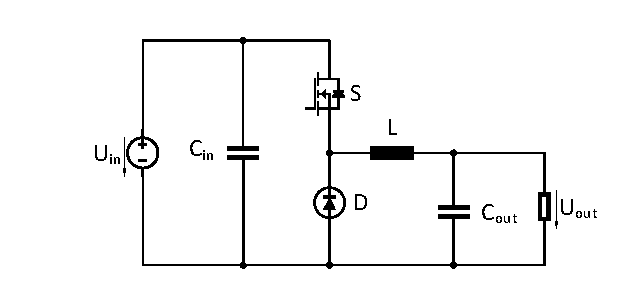
\includegraphics[width=0.9\linewidth]{content/Grafiken/Buck}
			\caption[Tiefsetzsteller]{Tiefsetzsteller}
			\label{fig:buck}
		\end{figure}
		Die Speicherdrossel des Tiefsetzstellers kann nach der Formel \ref{eq:BuckL} ausgelegt werden, wobei der gewünschte Stromrippel $\Delta I $ in der Drossel beispielhaft auf maximal 30 Prozent des \gls{Ia} festgelegt wird \cite{schmidtwalter}.
		\begin{equation}
			\label{eq:BuckL}
			L=\dfrac{U_{emax}-U_{a}}{f\cdot \Delta I}\cdot \dfrac{U_{a}}{U_{emax}} = \dfrac{U_{emax}-U_{a}}{f\cdot 0,3 \cdot I_{a}}\cdot \dfrac{U_{a}}{U_{emax}}
		\end{equation}
		Wird die Eingangsspannung durch einen dreiphasigen Diodengleichrichter, wie in Abb. \ref{fig:B6DiodRect} dargestellt,  implementiert, so kann die Eingangsspannung mit $U_{LL} \cdot \sqrt{2}$ berechnet werden. Daraus ergibt sich die Formel \ref{eq:BuckLB6} bezogen auf die Phasenspannungen. \\
		\begin{equation}
			\label{eq:BuckLB6}
			L=\dfrac{U_{LL} \cdot \sqrt{2}-U_{a}}{f\cdot 0,3 \cdot I_{a}}\cdot \dfrac{U_{a}}{U_{LL} \cdot \sqrt{2}}
		\end{equation}
		Außerdem gibt es die Möglichkeit des Interleavings, was die Verschachtelung der Schaltungen bedeutet also die Verbindung mehrerer Schaltungen zu einer. Die Taktung der Halbleiter wird versetzt ausgeführt und benötigt eine gekoppelte Steuerung. Dadurch können einerseits die Drosseln besser ausgenutzt und andererseits die Welligkeit des \gls{Ia} halbiert werden. 
		
		
		\subsection{Power Factor Correction (PFC)}
		Die \gls{PFC} ist eine notwendige Maßnahme, um den Blindleistungsanteil im Netz zu reduzieren und ist daher in heutigen Geräten standardmäßig implementiert. Ein Beispiel aus der Industrie, bei dem eine einfache Blindleistungskompensation bereits realisiert wurde, sind Leuchten mit Halogenlampen. Diese waren mit einem Transformator zur Erzeugung der notwendigen Spannung ausgestattet, der jedoch Blindleistung verursachte, was durch einfaches Hinzufügen eines Kondensators optimiert werden konnte. \\
		In herkömmlichen Gleichrichtersystemen werden getrennte Einheiten, bestehend aus einer dreiphasigen PFC-Gleichrichterschaltung und einem Gleichspannungswandler (DC/DC-Buck-Wandler), eingesetzt, um die Anforderungen zu erfüllen. Die Regelung der beiden Wandlerstufen erfolgt in der Regel entkoppelt, wobei der Gleichrichter sinusförmige Netzströme aufnimmt und der nachfolgende DC/DC-Wandler die Spannung an die erforderliche Ausgangsspannung anpasst. Das Streben nach kompakten und leichten Systemen erfordert hohe Schaltfrequenzen, die jedoch zu erhöhten Schaltverlusten und verringertem Wandlerwirkungsgrad führen können. Um dieses Problem zu lösen, können fortgeschrittene Modulationstechniken wie die Einfügung der dritten Harmonischen und Raumzeigermodulation eingesetzt werden. Alternativ kann die diskontinuierliche Pulsweitenmodulation (DPWM) als Methode zur Reduzierung der Schaltverluste in dreiphasigen PFC-Gleichrichtern eingesetzt werden, um sinusförmige Eingangsströme und eine konstante Gleichspannung zu gewährleisten. Im Gegensatz dazu müssen einstufige Umrichtersysteme beide Anforderungen gleichzeitig erfüllen, während zweistufige Systeme eine konstante Ausgangsspannung trotz niederfrequenter Spannungsschwankungen im Gleichspannungszwischennetz gewährleisten können.			
		\subsection{Leistungshalbleiter}
		Halbleiter sind prinzipiell alle Bauelemente mit mindestens einem PN-Übergang; können sie größere Leistungen schalten, werden sie als Leistungshalbleiter bezeichnet. Dabei sind für die verwendete Topologie neben der klassischen Diode vor allem \gls{MOSFET} relevant. Diese verdrängen derzeit in der Leistungselektronik häufig den verbreiteten IGBT aufgrund der preiswerter gewordenen Variante aus Siliziumkarbid \cite{SiCTrend}. Die Vorteile dieser neuen Technologie liegen in der Ermöglichung höherer Schaltfrequenzen, wodurch wiederum die in den induktiven Bauelementen zu speichernde Energie reduziert und somit Kosten eingespart werden können.\\
		Zur Auswahl der am besten geeigneten Halbleiter werden unter anderem Schaltungssimulationen eingesetzt, diese erfordern eine Nachbildung der Halbleiter. Um die Modelle der Leistungshalbleiter zu erstellen und ggf. vorhandene Modelle zu validieren, können Messungen im \gls{DPT} durchgeführt werden. Ein Beispiel für die in \gls{PLECS} implementierten Ausschaltverluste eines Halbleiters zeigt Abb. \ref{fig:plecsff2thermalmodel}. Es ist zu erkennen, dass die Punkte nur für den Betriebspunkt von 600 Volt zur Verfügung stehen, für andere Betriebsbereiche muss das Verhalten approximiert werden. Außerdem ist der \gls{RGV} nur für einen begrenzten Bereich dargestellt und die \gls{VGSS} nur auf einen Wert beschränkt. Dies kann in der späteren Anwendung zu deutlichen Abweichungen führen. 
		\begin{figure}
			\centering
			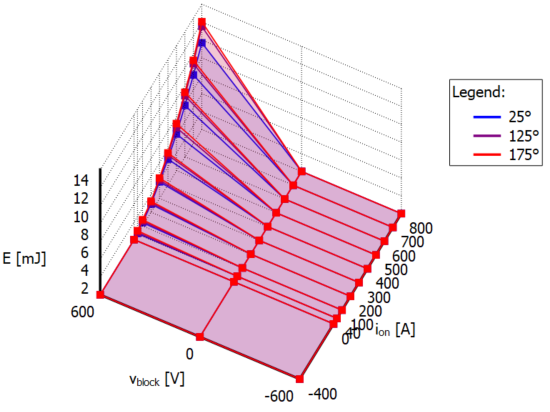
\includegraphics[width=0.7\linewidth]{content/Grafiken/PLECS_FF2ThermalModel}
			\caption{Darstellung der in PLECS implementierten Ausschaltverluste \cite{IFAGFF2}}
			\label{fig:plecsff2thermalmodel}
		\end{figure}
		
		\subsection{Induktive Komponenten}
		Induktive Bauelemente sind in der Regel Spulen und Transformatoren, die zur Speicherung und Übertragung von Energie dienen. Transformatoren bieten zusätzlich die Möglichkeit der galvanischen Entkopplung von Stromkreisen. 
		Für die Dimensionierung von Induktivitäten wird das Delta des Stromes in der Spule, der sogenannte Stromrippel, benötigt. Dieser Strom wird hier mit 30 Prozent des Effektivstroms ausgelegt. Für Drehstromsysteme kann der Rippelstrom nach der Formel \ref{eq:DeltaI} ermittelt werden. Dabei sind \gls{S} und \gls{Ull} die Spannungen zwischen den Außenleitern. \cite{Boge.2007}.\\
		\begin{equation}
			\label{eq:DeltaI}
			\Delta I = 0,3 \cdot \dfrac{\sqrt{2} \cdot S}{2 \cdot \sqrt{3} \cdot U_{LL}}
		\end{equation}
		Außerdem kann über die \gls{WL} eine Aussage über die Größe und damit indirekt über die Kosten und den Platzbedarf getroffen werden. Die Energie \gls{WL} kann mit der Formel \ref{eq:WL} berechnet werden. Dazu wird der Wert der Induktivität und der Effektivwert des Stroms $I_{RMS}$ benötigt \cite{Boge.2007}.
		\begin{equation}
			\label{eq:WL}
			W_{L} =\dfrac{1}{2}\cdot L\cdot I_{RMS}^{2}
		\end{equation}
				
			
\section{Integrated Active Filter Gleichrichter}
	Der \gls{IAF} Gleichrichter wurde erstmals 1997 in \cite{IAFfirst} für den Einsatz in Photovoltaikanwendungen vorgestellt. Er besteht aus einem Diodengleichrichter für den Hauptleistungspfad. Um sinusförmige Ströme in allen drei Phasen einzuprägen, wird dieser durch ein Netzwerk aus bidirektional sperrenden Leistungshalbleitern mit einer Induktivität und einer Halbbrücke, der sogenannten THI-Schaltung, ergänzt. Durch die Integration des Filters in den Leistungspfad ist keine externe Blindleistungskompensation erforderlich und die Filter können kleiner dimensioniert werden. Aufgrund des ungesteuerten Diodengleichrichters ist jedoch eine nachträgliche Spannungsregelung durch einen Tiefsetzsteller erforderlich \cite{ThesisSchrittwieserBuckTypePFC_2017}.\\
	Das Netzwerk aus bidirektionalen Schaltern, auch \gls{IVS} genannt, ermöglicht das Umschalten zwischen den einzelnen Phasen, in die durch die Induktivität und die Halbbrücke der gewünschte sinusförmige Stromverlauf eingeprägt wird. Dazu schaltet die Halbbrücke hinter der Induktivität entweder auf das positive oder auf das negative Potential der \gls{Upn}. Da der Diodengleichrichter immer nur aus zwei Phasen Strom bezieht, prägt die Schaltung ohne Phasenverschiebung nur in die jeweils dritte Phase Strom ein. Der \gls{IVS} schaltet mit Netzfrequenz und benötigt bidirektionale Schalter, um den Stromfluss während der gesamten Sinusperiode steuern zu können. Bei der Blindleistungsbereitstellung kommt es aufgrund der Phasenverschiebung zu einer Verschiebung zwischen Phasenstrom und Spannung. Dadurch ändert sich der Stromverlauf in der Drossel von einer Dreiecksfunktion ohne Blindleistung zu einer gekrümmten Funktion.
	\begin{figure}
		\centering
		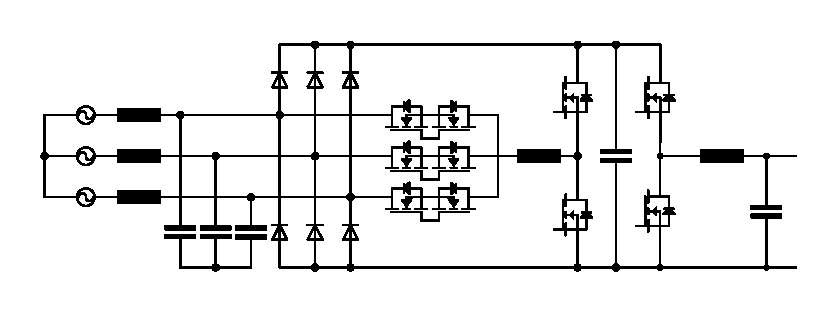
\includegraphics[width=0.9\linewidth]{content/Grafiken/IAF}
		\caption{\gls{IAF} Gleichrichter Topologie mit Tiefsetzsteller}
		\label{fig:iaf}
	\end{figure}


\section{B6-1/3-PWM PFC Gleichrichter}
	\label{sec:GrundlagenB6}
	Diese Topologie ist eine weit verbreitete B6-Topologie, die aus drei Halbbrücken besteht, die jeweils an eine Phase angeschlossen sind. Durch ein adaptives Modulationsverfahren unter Verwendung von Induktivitäten auf der Netzseite werden die Schaltverluste und \gls{SDL} reduziert. Das Verfahren wurde von Menzi, Bortis und Kolar \cite{13PWMPFC} ausführlich beschrieben. Zur Regelung der Ausgangsspannung wird ein entkoppelter Tiefsetzsteller verwendet.\\
	
	\begin{figure}
		\centering
		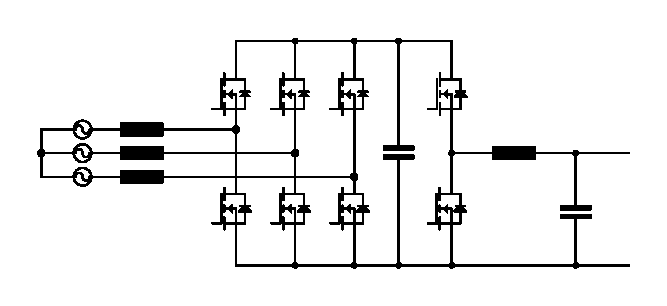
\includegraphics[width=0.9\linewidth]{content/Grafiken/B6_Buck}
		\caption[1/3 PWM PFC Topologie mit Tiefsetzsteller]{1/3 PWM PFC Topologie mit Tiefsetzsteller}
		\label{fig:b6buck}
	\end{figure}
	
	Die Besonderheit der Regelung besteht darin, dass die Phase, die gerade keinen Strom führt, weil sie die niedrigste Spannung hat, durch \gls{PWM} Ansteuerung der entsprechenden Halbbrücke einen entsprechenden Stromfluss erhält. Die beiden anderen Halbbrücken werden jeweils wie ein Diodengleichrichter geschaltet. Dieser Vorgang ist prinzipiell der gleiche wie beim \gls{IAF} und kann daher zum besseren Verständnis gemeinsam betrachtet werden, siehe Abb. \ref{fig:b6iafsectors}.
	Im hervorgehobenen Abschnitt ist das Potential der Phase b am niedrigsten und man sieht im Bereich (f), dass nur eine Halbbrücke durch \gls{PWM} angesteuert wird. In Bereich (e) ist der Tastgrad \gls{D} dargestellt, wobei der Wert 1 die permanente Verbindung mit dem positiven Potential und -1 die Verbindung mit dem negativen Potential des Zwischenkreises \gls{Upn} darstellt \cite{13PWMPFC}.\\ 
		
	\begin{figure}
		\centering
		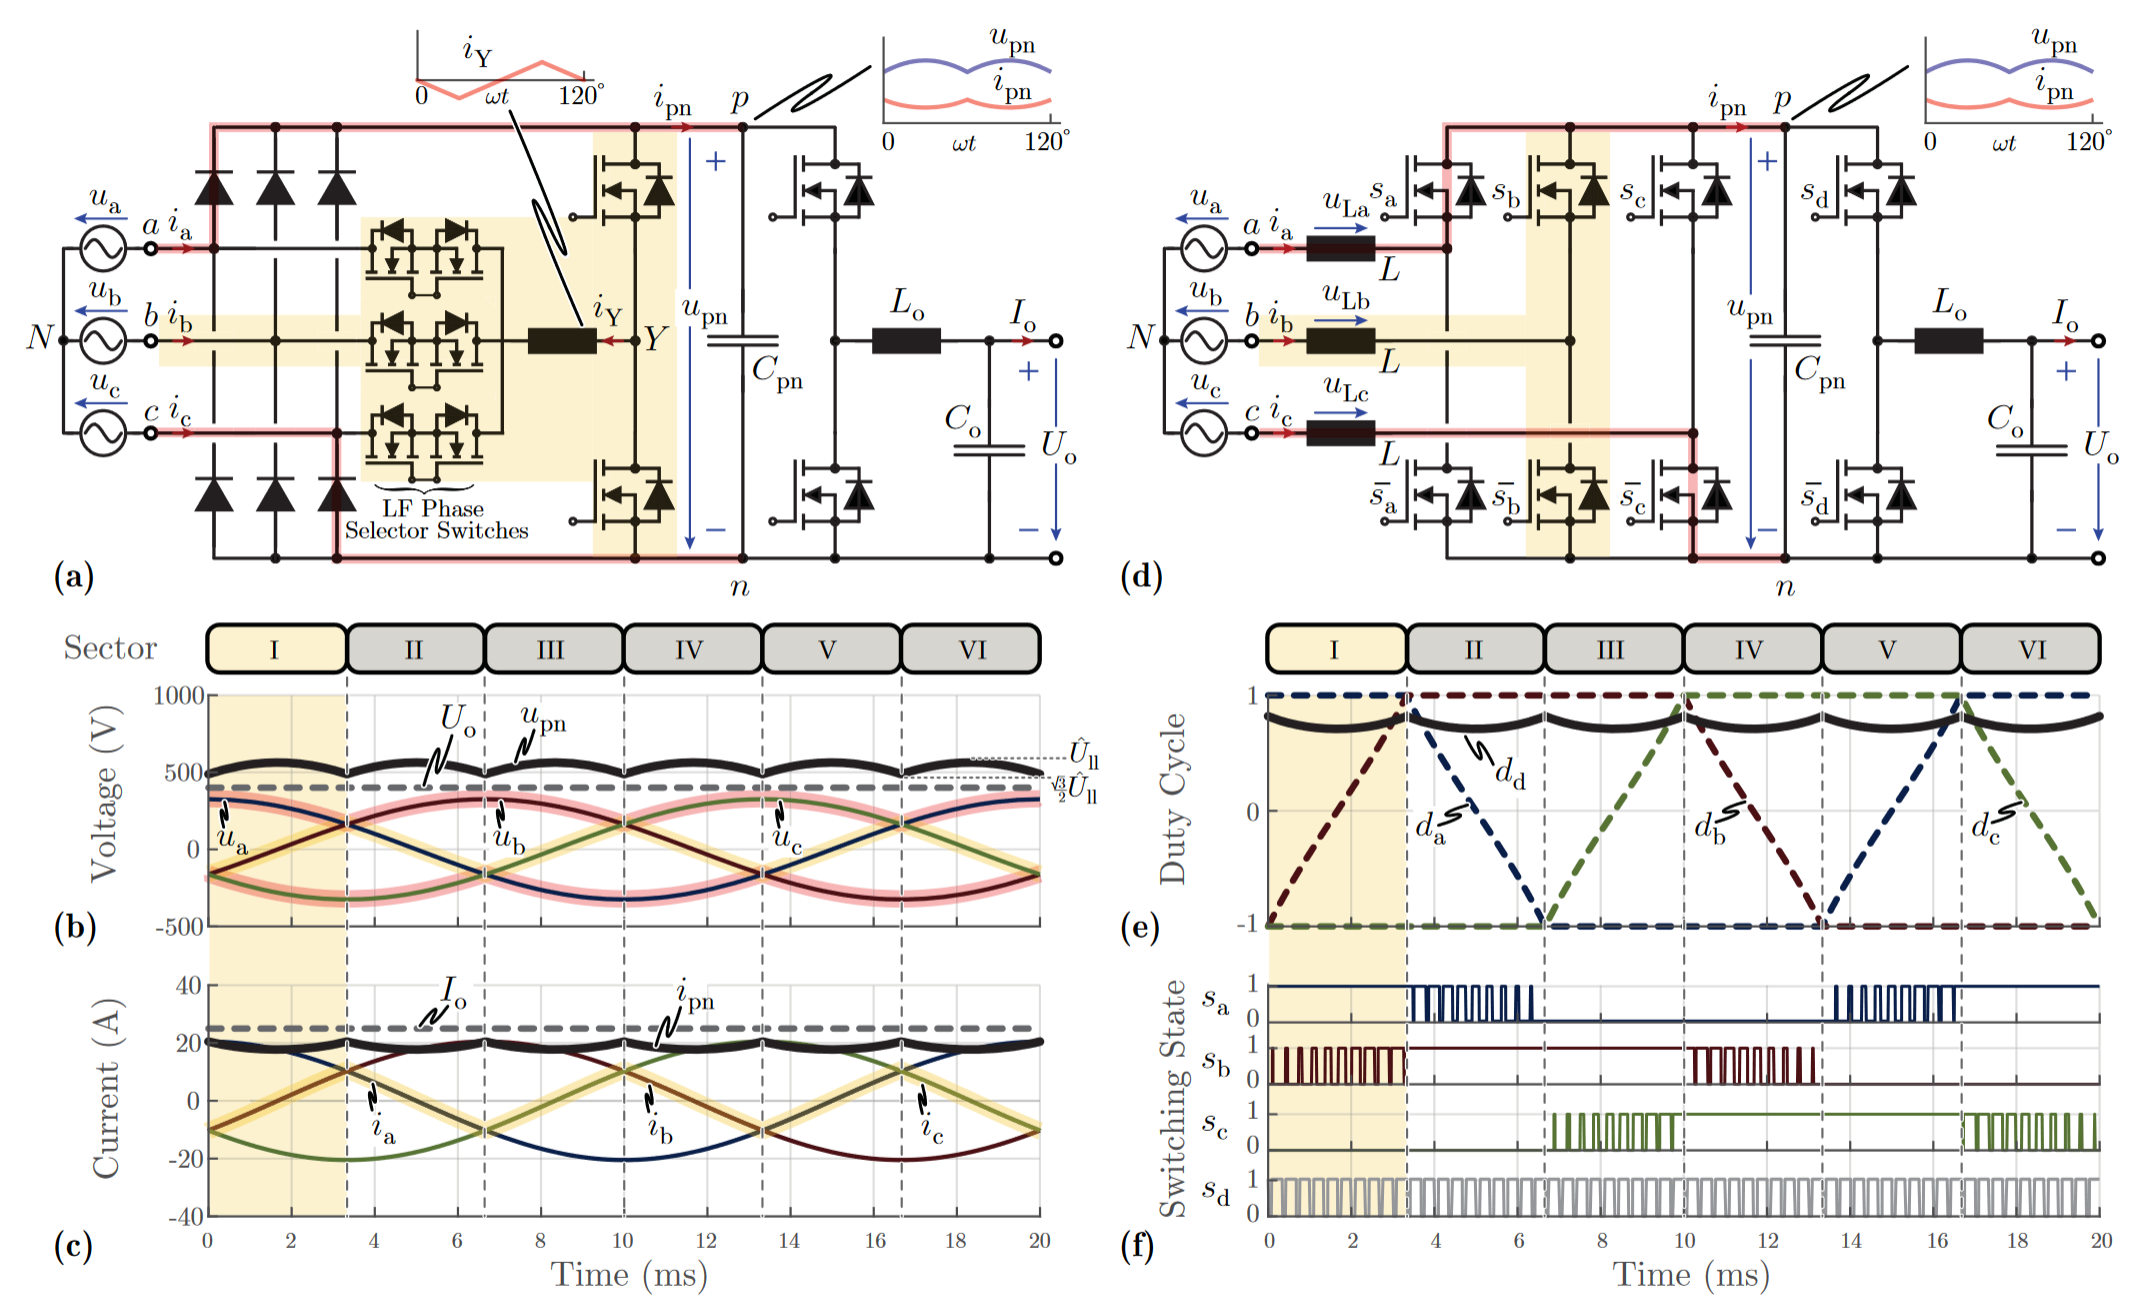
\includegraphics[width=1\linewidth]{content/Grafiken/B6+IAF_Sectors.png}
		\caption{Sektorenaufteilung und Schaltverhalten von IAF und B6 1/3 \cite{13PWMPFC}}
		\label{fig:b6iafsectors}
	\end{figure}





\section{Simulationssoftware}
	Um die Machbarkeit von Topologien bewerten und untersuchen zu können, ist es notwendig, diese in einer Gesamtsimulation zu betrachten. Dies ermöglicht es, die Funktionalität und den Einfluss der Parameter im direkten Zusammenspiel zu untersuchen. Insbesondere das Verhalten für Systemdienstleistungen, wie die Phasenverschiebung und die dadurch beeinflusste Verteilung der Verlustleistungen, soll als Entscheidungsgrundlage dienen.\\
	Es wird die Version R2022a von Matlab mit Simulink Version 10.5 und Plecs Version 4.6.8 verwendet.  

	\subsection{PLECS}
	Die Software \gls{PLECS} der Firma PLEXIM wird als Integration in MATLAB mit Simulink verwendet.  Sie ermöglicht die Modellierung von Schaltungen unter Berücksichtigung des thermischen Verhaltens durch elektrische Verlustleistungsmodelle. Dazu wird die Energie im Schaltvorgang sowie im durchgeschalteten Zustand in der Schaltung berücksichtigt. Dies ermöglicht die Betrachtung der Verlustleistung innerhalb des Halbleiters und damit den Aufwand für die Kühlung und eine Abschätzung des Wirkungsgrades der Schaltung. Ein Beispiel der Funktionen ist in Abb. \ref{fig:plecsbuck} zu sehen, die thermische Kette muss aus Datenblättern o.ä. der Kühlkörper bekannt sein. Für Halbleiter werden thermische Modelle benötigt, die ebenfalls aus Datenblättern erstellt oder vom Hersteller zur Verfügung gestellt werden können. Allerdings gibt es nicht für alle Halbleiter ausreichende Informationen und die tatsächliche Verlustleistung hängt von vielen Parametern ab. Daher ist es oft notwendig, eigene Messungen durchzuführen, um die spätere Anwendung bestmöglich simulieren zu können. In den verwendeten Modellen der Leistungshalbleiter wird die Thermische Kette bereits im Modell berücksichtigt und muss daher nicht als externer Block wie in Abbildung \ref{fig:plecsbuck} berücksichtigt werden. Außerdem werden die Zeitlichen Konstanten in den Modellen verringert, um schneller einen eingeschwungenen Zustand zu erreichen. \\
	
	\begin{figure}
		\centering
		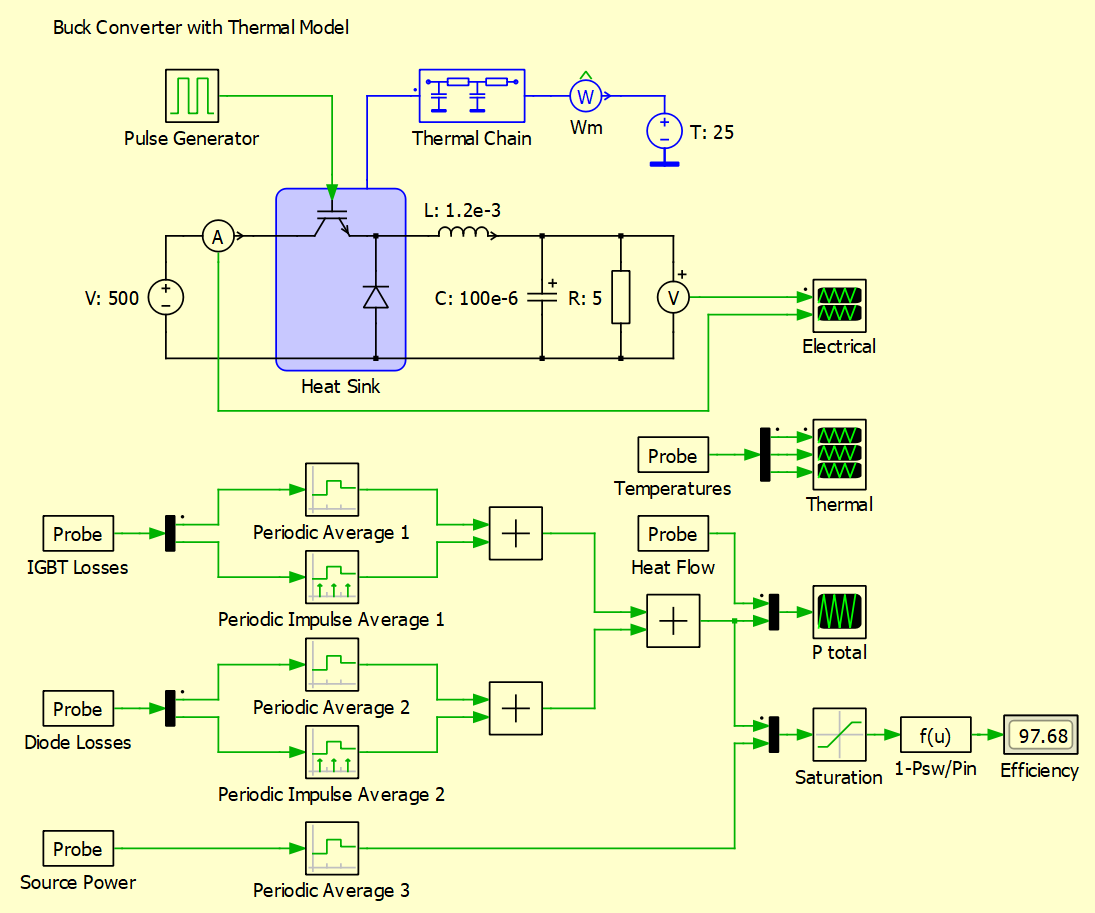
\includegraphics[width=1\linewidth]{content/Grafiken/PLECS_Buck}
		\caption[Tiefsetzsteller mit Effizienzbestimmung]{Tiefsetzsteller mit Effizienzbestimmung}
		\label{fig:plecsbuck}
	\end{figure}
	